\section{Experimental Setup}

This section contains the hardware setup used to communicate with the low cost IMU sensors and the platform that the Kalman filter is implemented on. There were two Inertial
Navigation Systems (INS) used to compare the results of the implemented Kalman filter to,
the MIDGII and the UmarimLite. The MIDGII is an expensive INS known as the golden
standard for AHRS and the UmarimLite is a commercially available low-cost AHRS that
uses the open source Paparazzi autopilot software. The experimental setup was chosen such
that the algorithm could be designed and tested without any of the low-cost considerations, this makes it possible to develop the algorithm with no constraints and then optimize the
algorithm for low-cost systems.

\subsection{Hardware}

As our projected solution involved a low-cost navigation system, the hardware selection criteria were primarily founded on availability and cost. The cost reduction normally concedes in accurateness and reliability, although with the recent surge of inexpensive, widely accessible, and precise microelectromechanical systems (MEMS), that is no longer the case. Still, we aim to employ commercially available tools at the lowest possible cost without compromising the design of a robust and accurate inertial navigation system. A LoPy microcontroller was selected as the navigational computing device of the inertial system, meeting the envisioned requirements for low power with flexible and diverse computational capabilities. The LoPy development board interfaces with the external physical inertial sensor through connection pins (figure \ref{fig:hardware}.a) and communicates remotely by LoRa protocol. A PySense expansion board connects with the LoPy module providing a programable interface for the microcontroller. The inertial navigation system encompasses a small MPU-9250 (figure \ref{fig:hardware}.b)

\begin{figure}[!h]
    \centering
    \begin{subfigure}{0.49\textwidth}
        \centering
        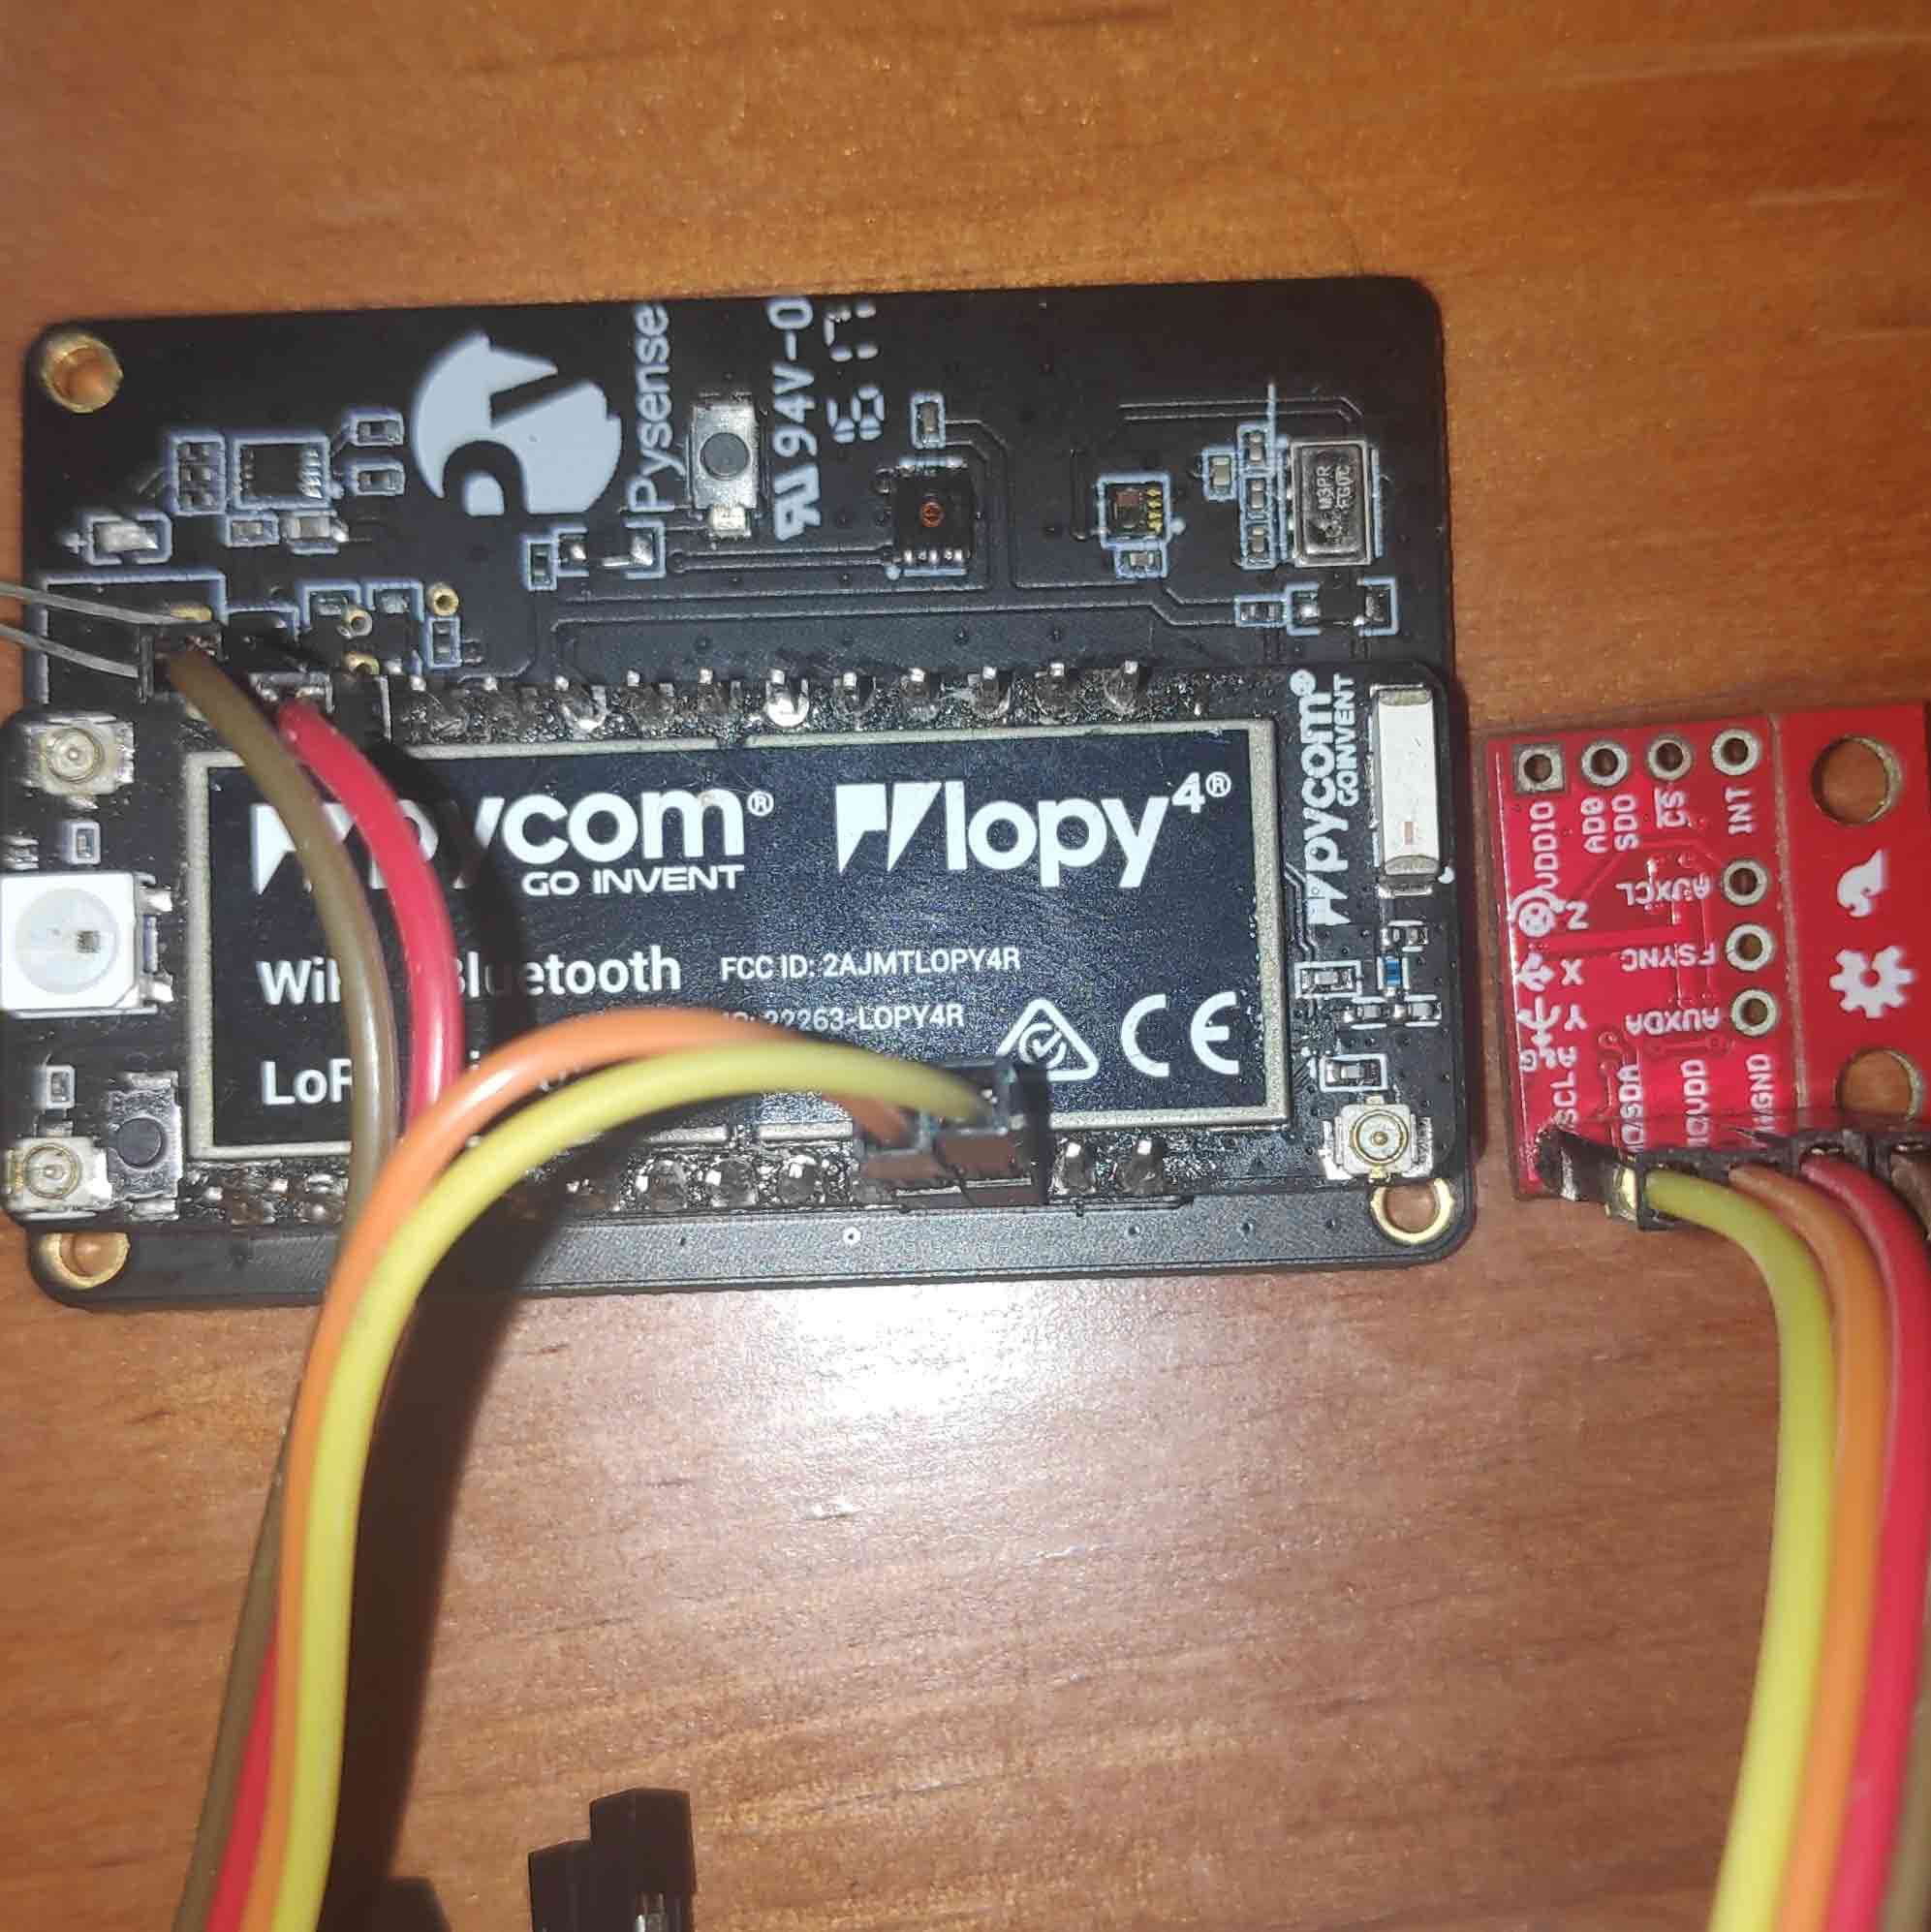
\includegraphics[width=1\textwidth]{figures/INS.jpg}
        \caption{INS Hardware}
        \label{fig:sub1}
    \end{subfigure}%
    \begin{subfigure}{0.49\textwidth}
        \centering
        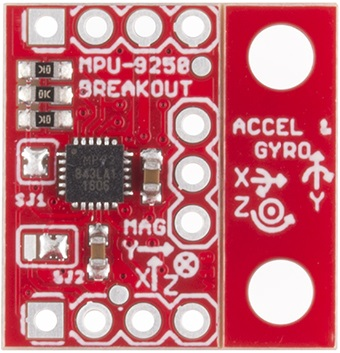
\includegraphics[width=1\textwidth]{figures/mpu9250.jpg}
        \caption{MPU-9250 Breakout}
        \label{fig:sub2}
    \end{subfigure}
    \caption{Pin connection between the microcontroller (left) and the IMU (right). Modules are linked through SCL, CLK, VDD and GND pins.}
    \label{fig:hardware}
\end{figure}

MPU-9250 inertial measurement unit is one of the most widely available low cost commercial IMUs. It is also considered to have an exceptional quality price ratio. The MPU-9250 contains as well temperature and pressure sensors. This chip is extensively employed in wearable sensors for health, fitness, and sports, motion-based game controllers, and portable gaming. This IMU is operated to estimate motion by identifying the presence of acceleration vectors, rotational rates, and local magnetic field direction. It features an embedded 9-axis MEMS sensor from InvenSense. The MPU-9250 is a combined System-in-package (SIP) comprising an MPU-6500 (3-axis accelerometer and 3-axis gyroscope combination) and an AK8963 3-axis magnetometer.

\subsubsection{Accelerometer}

The triple-axis MEMS accelerometer in MPU-9250 includes a wide range of features:

\begin{itemize}
    \item Digital-output triple-axis accelerometer with a programmable full scale range  of $\pm 2g$, $\pm 4$, $\pm 8g$ and $\pm 16g$ and integrated 16-bit ADCs
    \item Accelerometer normal operating current: $450 \mu A$
    \item The text in the entries may be of any length
    \item Low power accelerometer mode current: $8.4 \mu A$ at $0.98Hz$, $19.8 \mu A$ at 31.$25Hz$
    \item Sleep mode current: $8 \mu A$
    \item User-programmable interrupts
    \item Wake-on-motion interrupt for low power operation of applications processor
    \item Self-test
\end{itemize}

\begin{table}[H]
    \begin{center}
        \begin{tabular}[t]{lcccc}
            \hline
            Parameter                   & Min. & Typ.      & Max.   & Units             \\
            \hline
            Full-Scale range            &      & $\pm 16$  &        & $g$               \\
            Sensitivity Scale Factor    &      & 2,048     &        & $LSB/g$           \\
            Nonlinearity                &      & $\pm 0.1$ &        & $\%$              \\
            Rate Noise Spectral Density &      & 300       &        & $\mu g/\sqrt{Hz}$ \\
            Operating Current           &      & 3.2       &        & $mA$              \\
            Startup Time                &      & 20        &        & $ms$              \\
            Output Data Rate            & $4$  &           & $4000$ & $Hz$              \\
            \hline
        \end{tabular}
        \caption{Accelerometer Specifications. }
        \label{tab:accelerometer_specification}
    \end{center}
\end{table}

\subsubsection{Gyroscope}

The triple-axis MEMS gyroscope in the MPU-9250 includes a wide range of features:

\begin{itemize}
    \item Digital-output X-Axis, Y-Axis, and Z-Axis angular rate sensors (gyroscopes) with a user-programmable fullscale range of $\pm 250$, $\pm 500$, $\pm 1000$, and $\pm 2000^{\circ}/s$ and integrated 16-bit ADCs
    \item Digitally-programmable low-pass filter
    \item Gyroscope operating current: $3.2mA$
    \item Sleep mode current: $8 \mu A$
    \item Factory calibrated sensitivity scale factor
    \item Self-test
\end{itemize}


\begin{table}[H]
    \begin{center}
        \begin{tabular}[t]{lcccc}
            \hline
            Parameter                   & Min. & Typ.       & Max.   & Units                  \\
            \hline
            Full-Scale range            &      & $\pm 2000$ &        & $^{\circ}/s$           \\
            Sensitivity Scale Factor    &      & 131        &        & $LSB/(^{\circ}/s)$     \\
            Nonlinearity                &      & $\pm 0.5$  &        & $\%$                   \\
            Rate Noise Spectral Density &      & 300        &        & $^{\circ}/s/\sqrt{Hz}$ \\
            Operating Current           &      & 450        &        & $\mu A$                \\
            Startup Time                &      & 35         &        & $ms$                   \\
            Output Data Rate            & $4$  &            & $8000$ & $Hz$                   \\
            \hline
        \end{tabular}
        \caption{Gyroscope Specifications. }
        \label{tab:gyroscope_specification}
    \end{center}
\end{table}

\subsubsection{Magnetometer}

The triple-axis MEMS accelerometer in MPU-9250 includes a wide range of features:
\begin{itemize}
    \item 3-axis silicon monolithic Hall-effect magnetic sensor with magnetic concentrator
    \item Wide dynamic measurement range and high resolution with lower current consumption.
    \item Output data resolution of 14 bit ($0.6 \mu T/LSB$) or 16 bit ($15 \mu T/LSB$)
    \item Full scale measurement range is $\pm 4800 \mu T$
    \item Magnetometer normal operating current: $280\mu A$ at $8 Hz$ repetition rate
    \item Self-test function with internal magnetic source to confirm magnetic sensor operation on end products
\end{itemize}

\begin{table}[H]
    \begin{center}
        \begin{tabular}[t]{lcccc}
            \hline
            Parameter                     & Min. & Typ.       & Max. & Units        \\
            \hline
            Full-Scale range              &      & $\pm 4800$ &      & $\mu T$      \\
            Sensitivity Scale Factor      &      & 0.6        &      & $\mu T/ LSB$ \\
            Operating Current             &      & 280        &      & $\mu A$      \\
            Initial Calibration Tolerance &      & $\pm 500$  &      & $LSB$        \\
            \hline
        \end{tabular}
        \caption{Magnetometer specification. }
        \label{tab:magnetometer_multiplication}
    \end{center}
\end{table}

\subsubsection{Calibration}

A correct calibration of such sensors is essential for the compensation of their systematic errors, bias, and scale factor. Each time prior to an experiment, the inertial sensor is calibrated while the system is stationary and stabilized to compensate for static error that might corrupt the measurements.


\subsection{Software}
The microcontroller operates MicroPython, a barebones and efficient implementation of Python 3, which incorporates a small subset of the Python standard library. It is optimized to run on microcontrollers and in constrained environments. The inertial module's raw measurements are interpreted by the microcontroller through Inter-Integrated Circuit (I2C) MicroPython driver serial allowing to read the peripherals memory addresses synchronously. The readings of each sensor are later averaged and linearized to better detect and reduce the presence of outlier readings. A fusion algorithm takes as input the averaged data of the accelerometer, gyroscope, and magnetometer. It returns the estimated inertial angles (pitch, roll, and yaw) as well as the projected linear acceleration with a gravity compensation numerical method that utterly removes the effect of the gravity component. Numerically integrating the resultant linear acceleration yields velocity, and double integrating will deliver the body's accumulative position. Merging the AHRS with an accumulative position allows tracking a moving body in three dimensions over time.

\subsection{System Architecture}
Moreover, the navigation system is equipped with a LoRa antenna enabling the system to transmit at 868MHz/915MHz LoRa bands in real-time at a long distance the position and orientation information to an external gateway (figure \ref{fig:overview}). A visualization of the entire hardware solution is provided at image \ref{fig:full}.

\begin{figure}[!h]
    \centering
    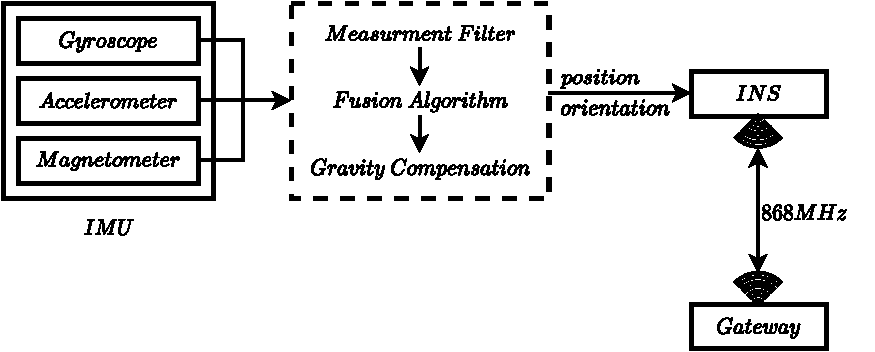
\includegraphics[width=0.9\textwidth]{figures/overview.pdf}
    \caption{System overview - Raw measurements from IMU are fused together and numerically integrated to obtain position and orientation. This INS data is transmitted in real-time to a remote node gateway. }
    \label{fig:overview}
\end{figure}

\subsection{Experiments}

\begin{figure}[!h]
    \centering
    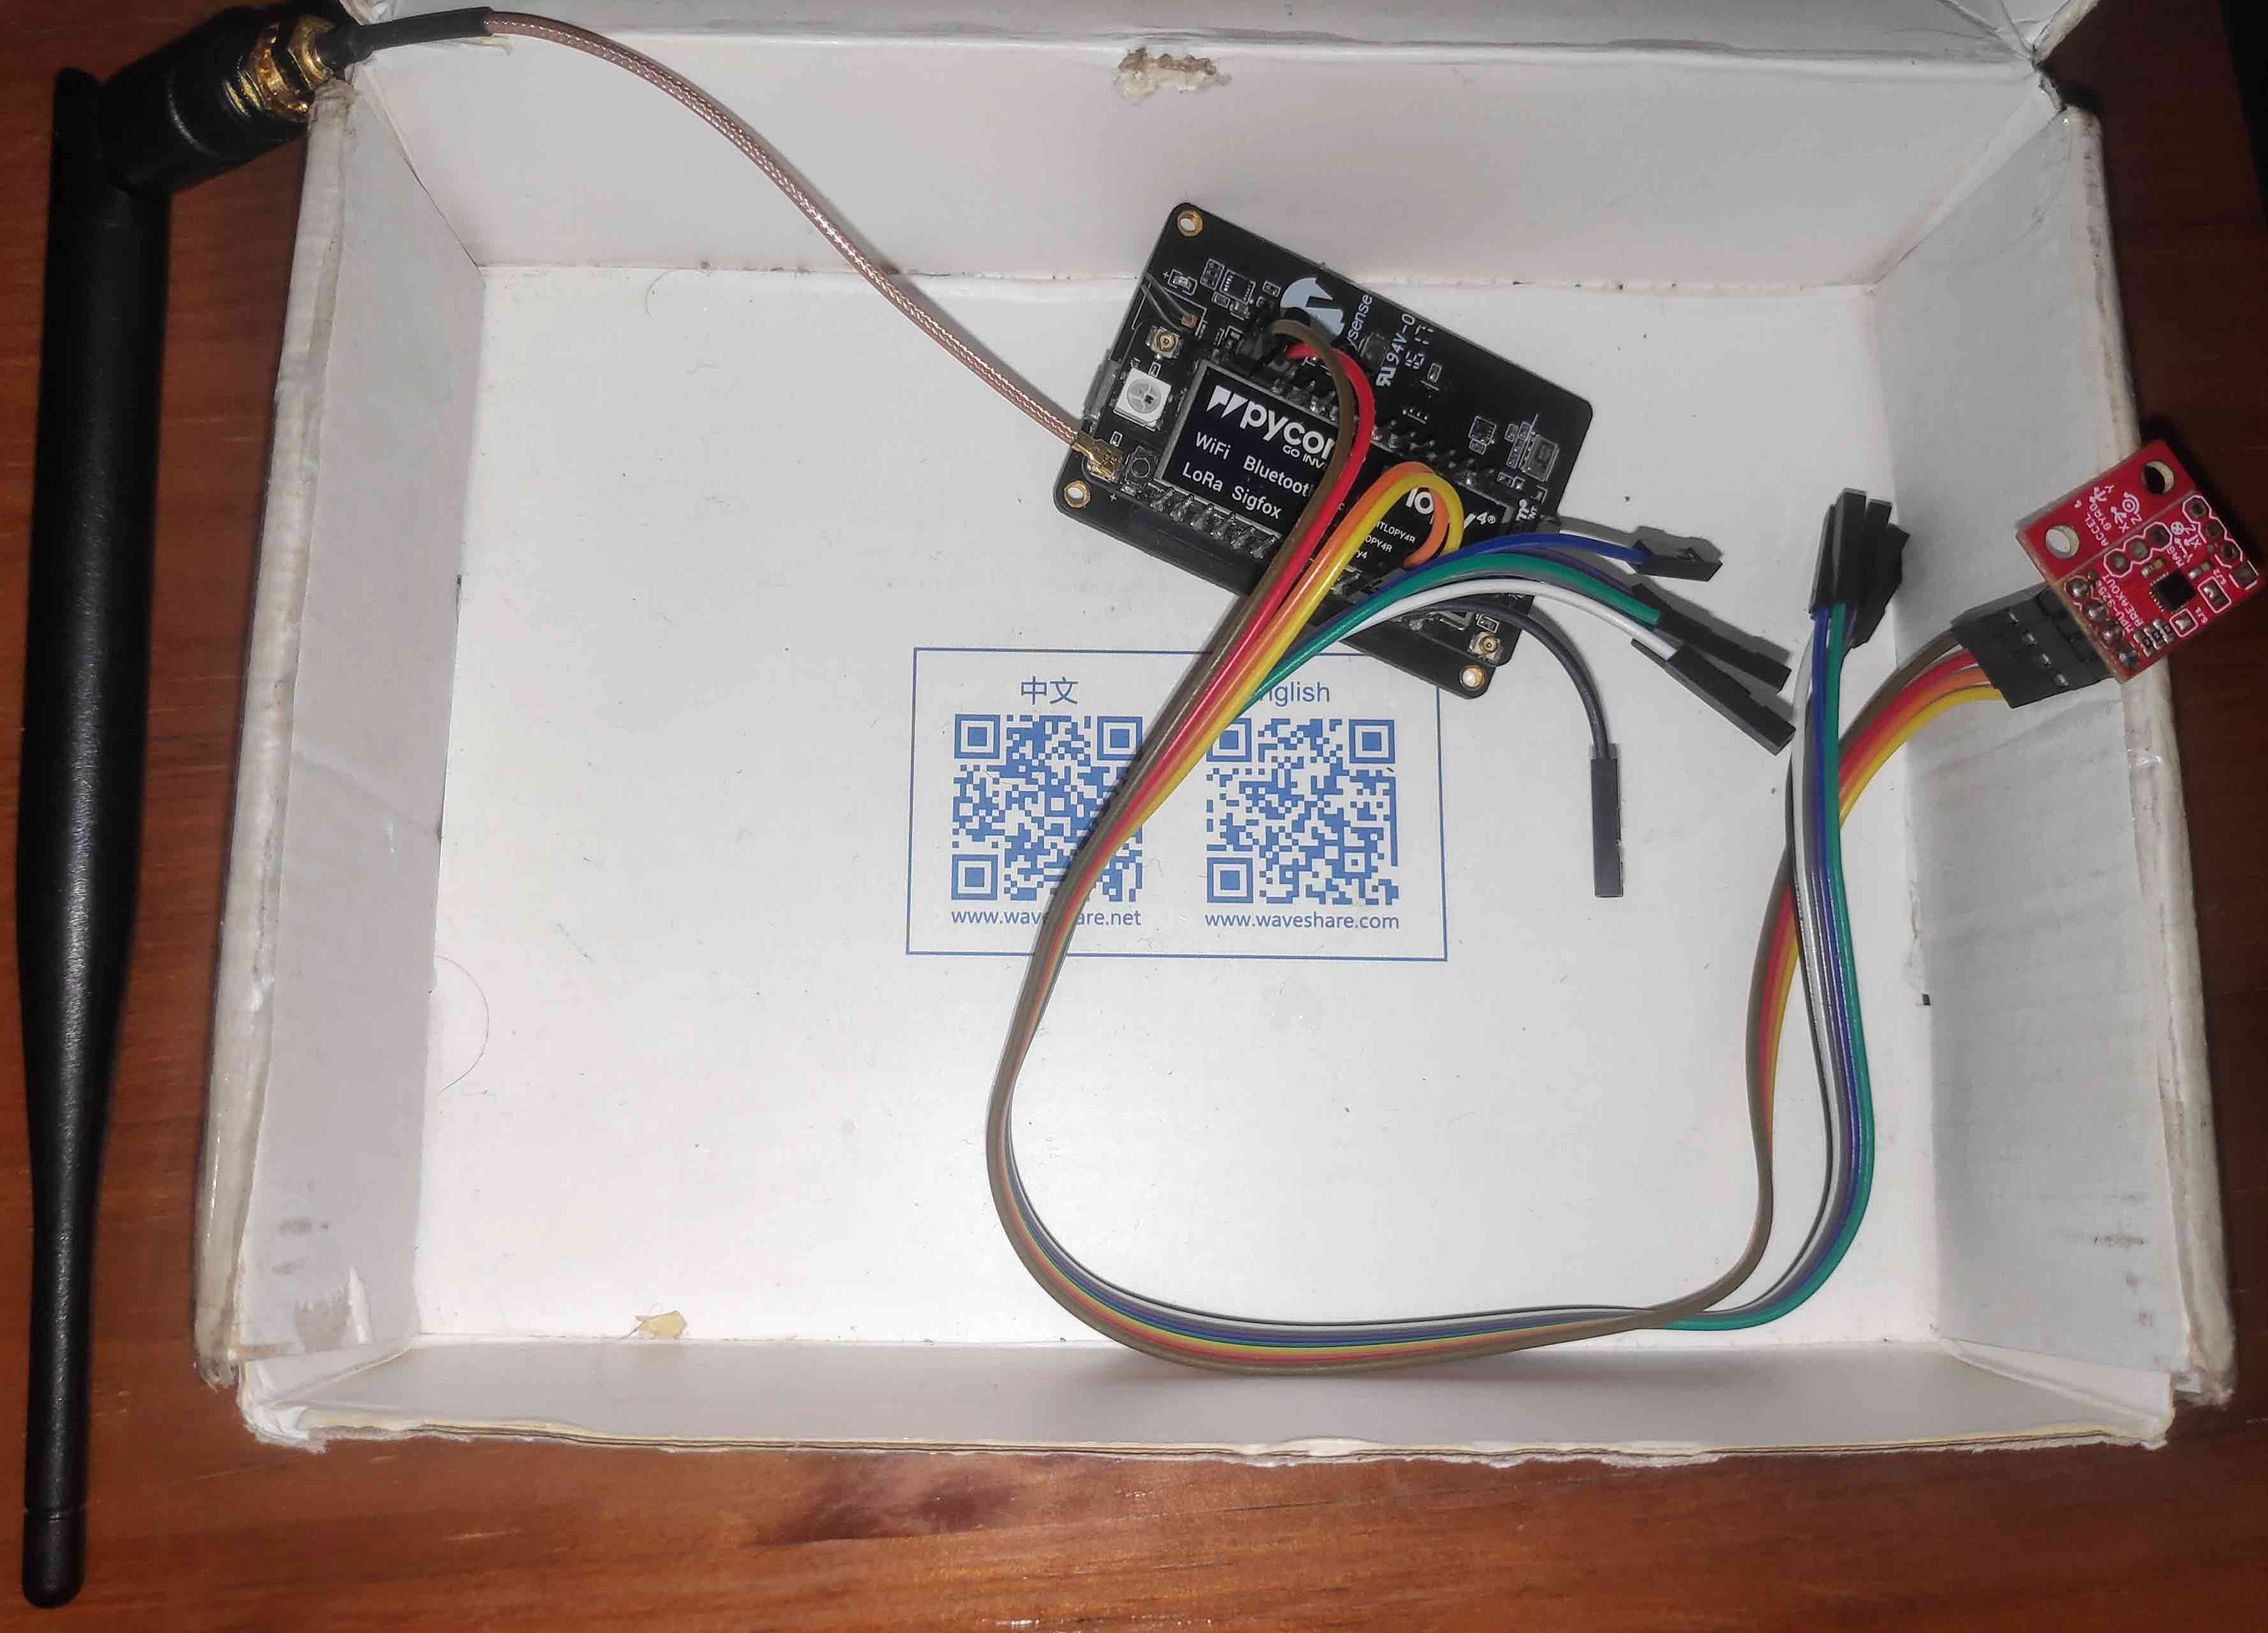
\includegraphics[width=0.9\textwidth]{figures/fullINS.jpg}
    \caption{Complete hardware solution - Box containing the full inertial navigation system, at the left the antenna  suitable for use in the 868MHz/915MHz LoRa bands. }
    \label{fig:full}
\end{figure}
\subsection{Indoor Experiments}
\begin{figure}[!h]
    \centering
    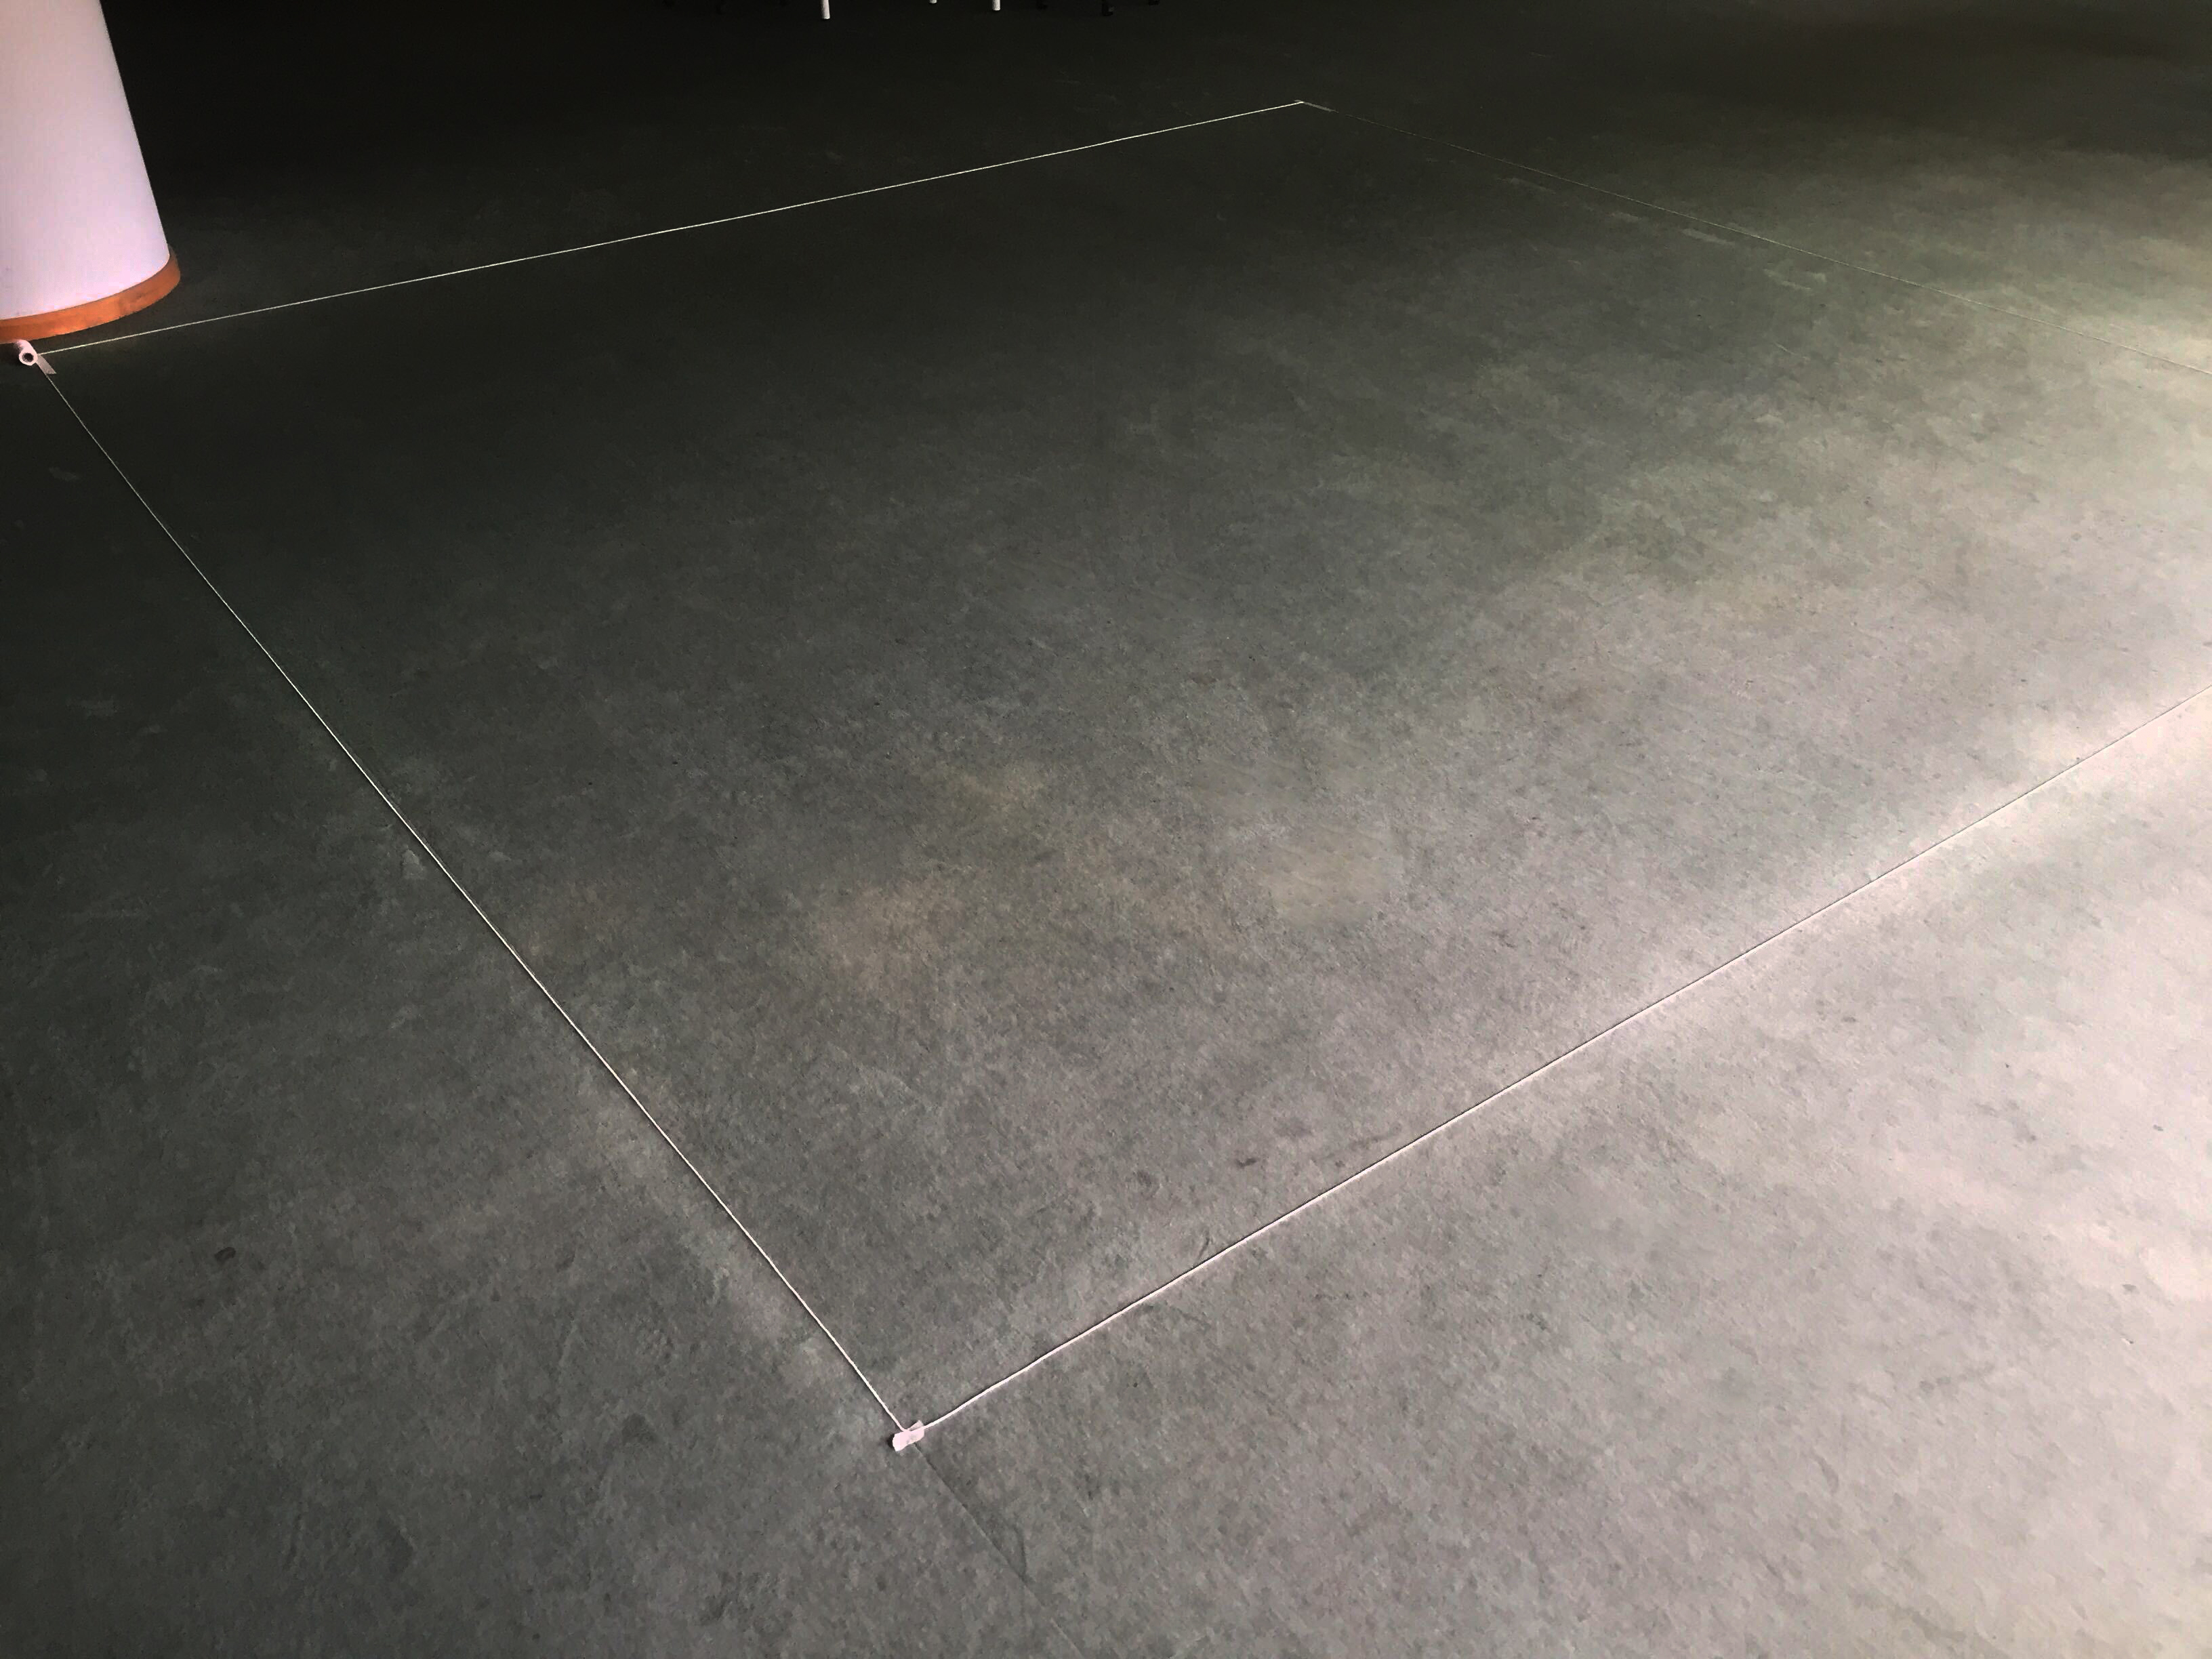
\includegraphics[width=0.9\textwidth]{figures/indoor.jpg}
    \caption{ 5 meter side ground square used for baseline of accuracy of inertial system. }
    \label{fig:indoor}
\end{figure}

\begin{figure}[!h]
    \centering
    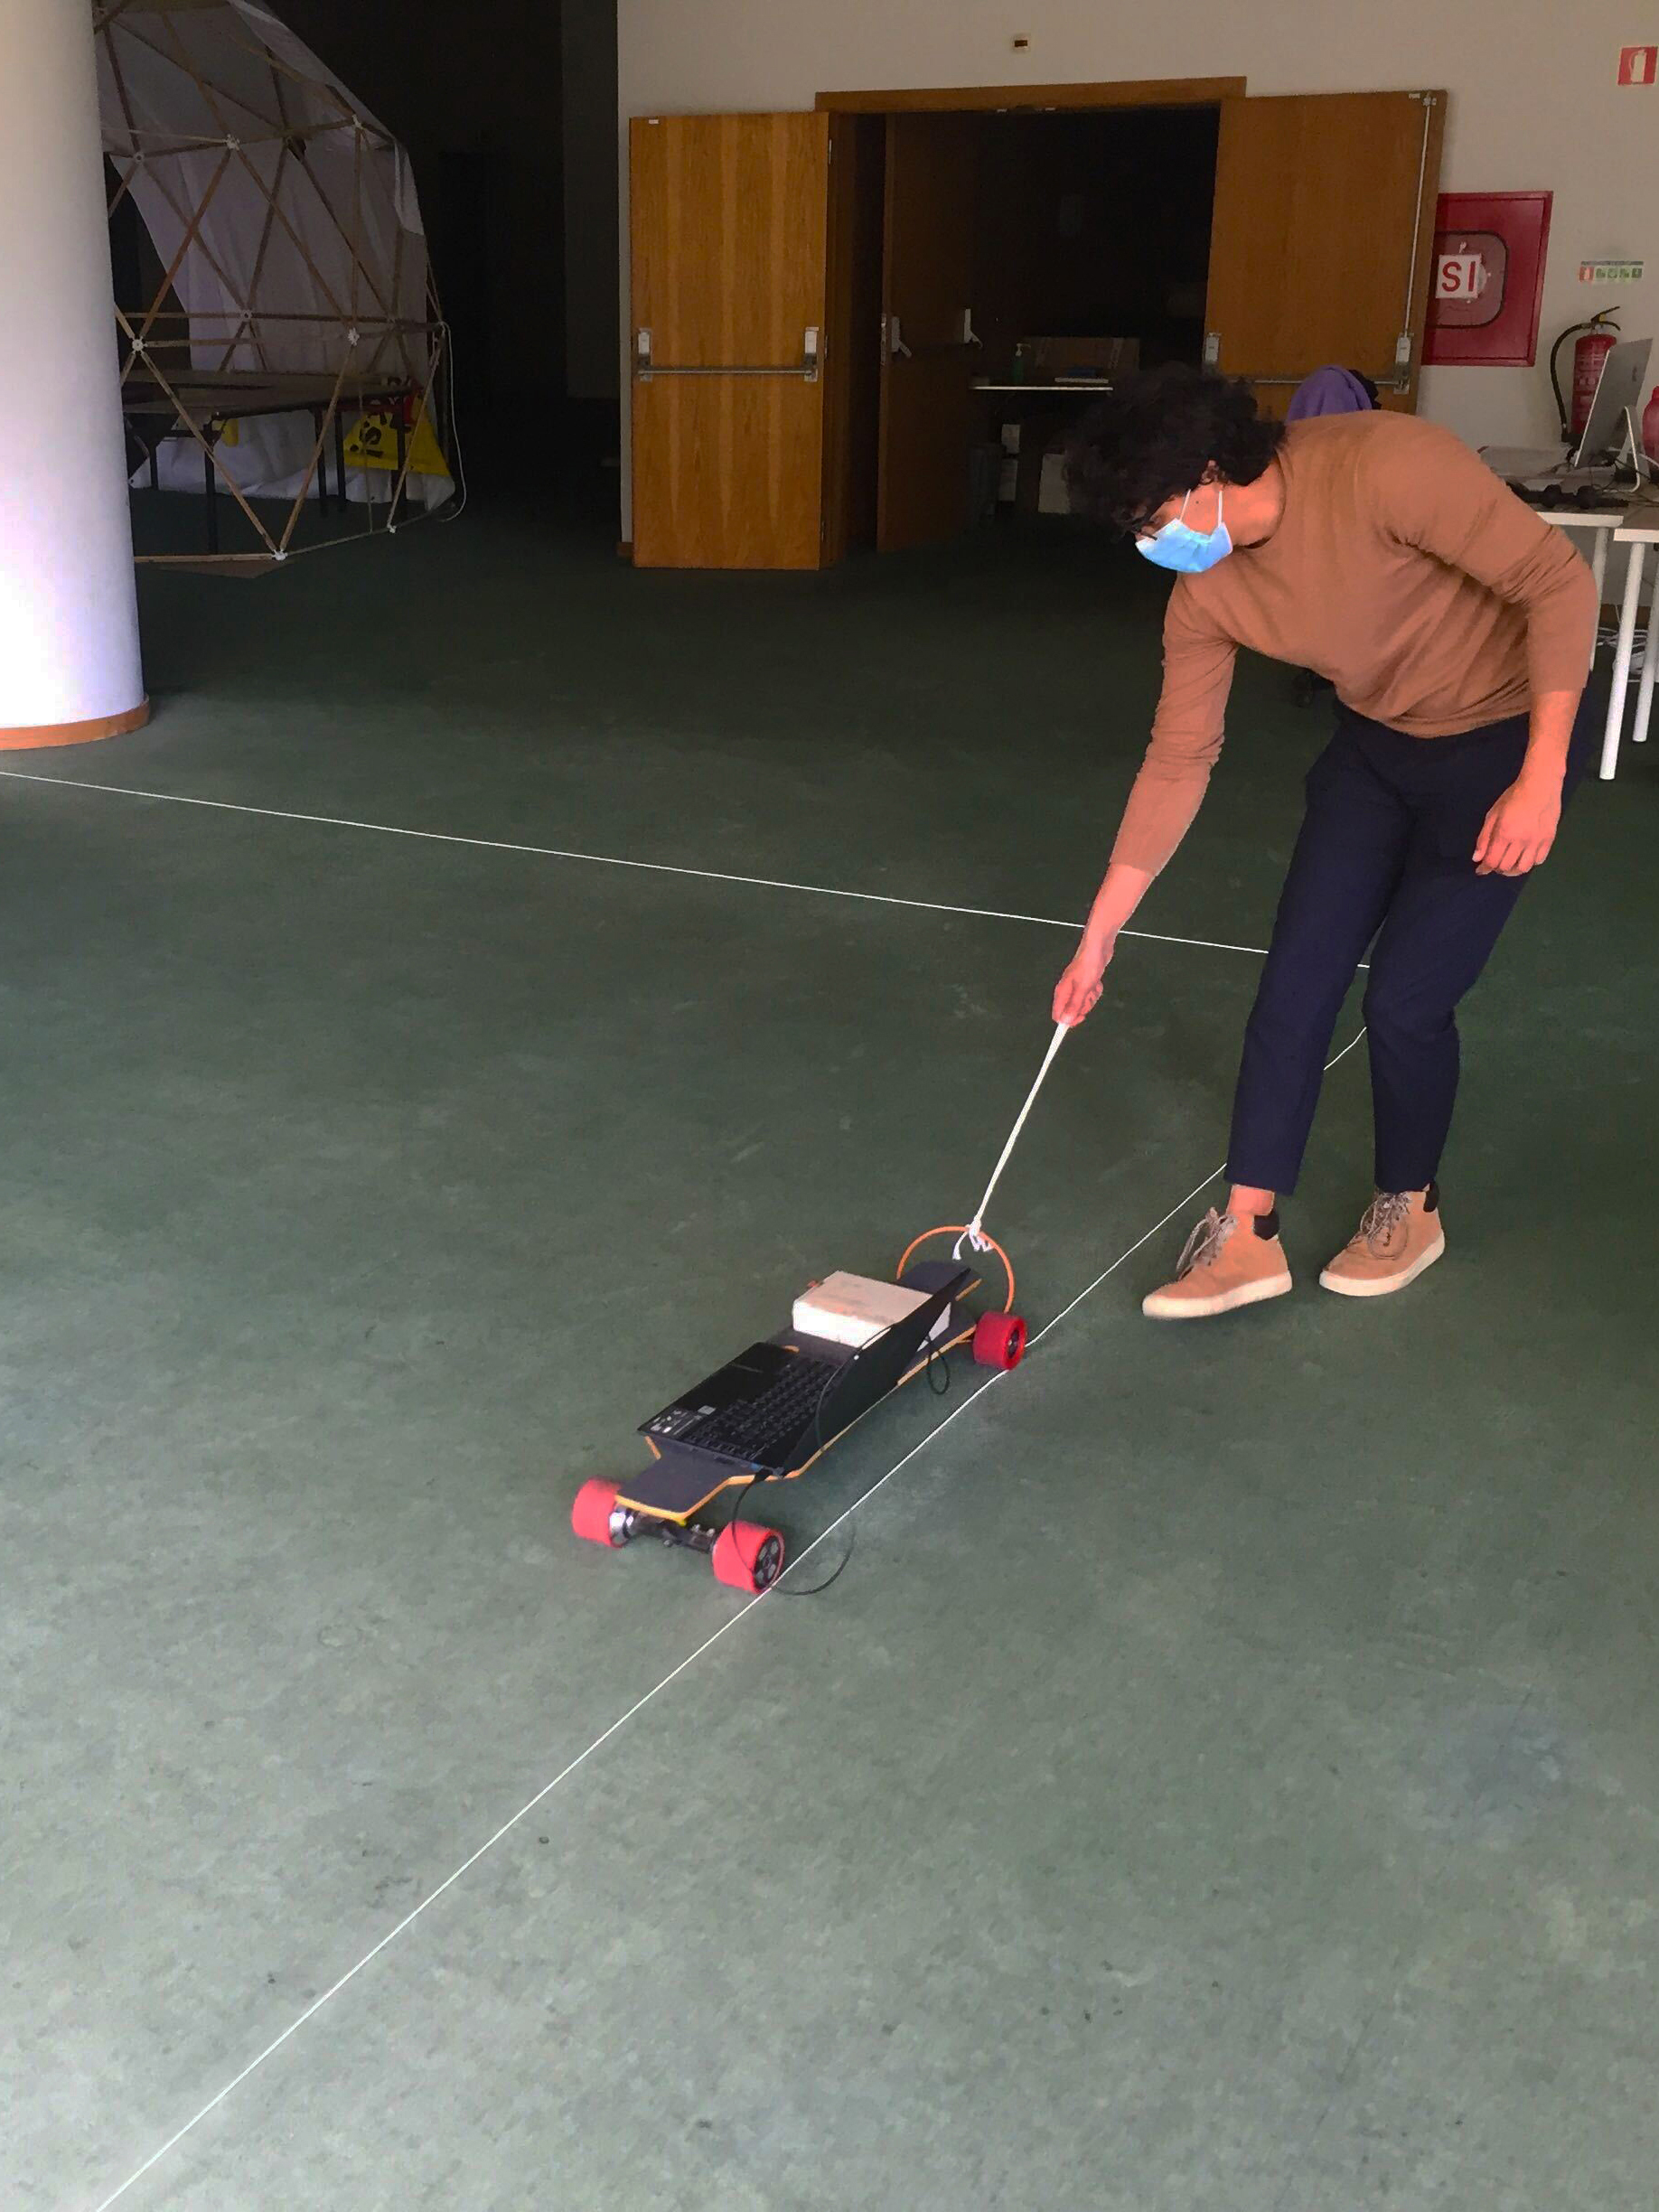
\includegraphics[width=0.9\textwidth]{figures/indoor_1.jpg}
    \caption{ Manually pulling the skateboard on each side of the ground square. }
    \label{fig:indoor_1}
\end{figure}

\begin{figure}[!h]
    \centering
    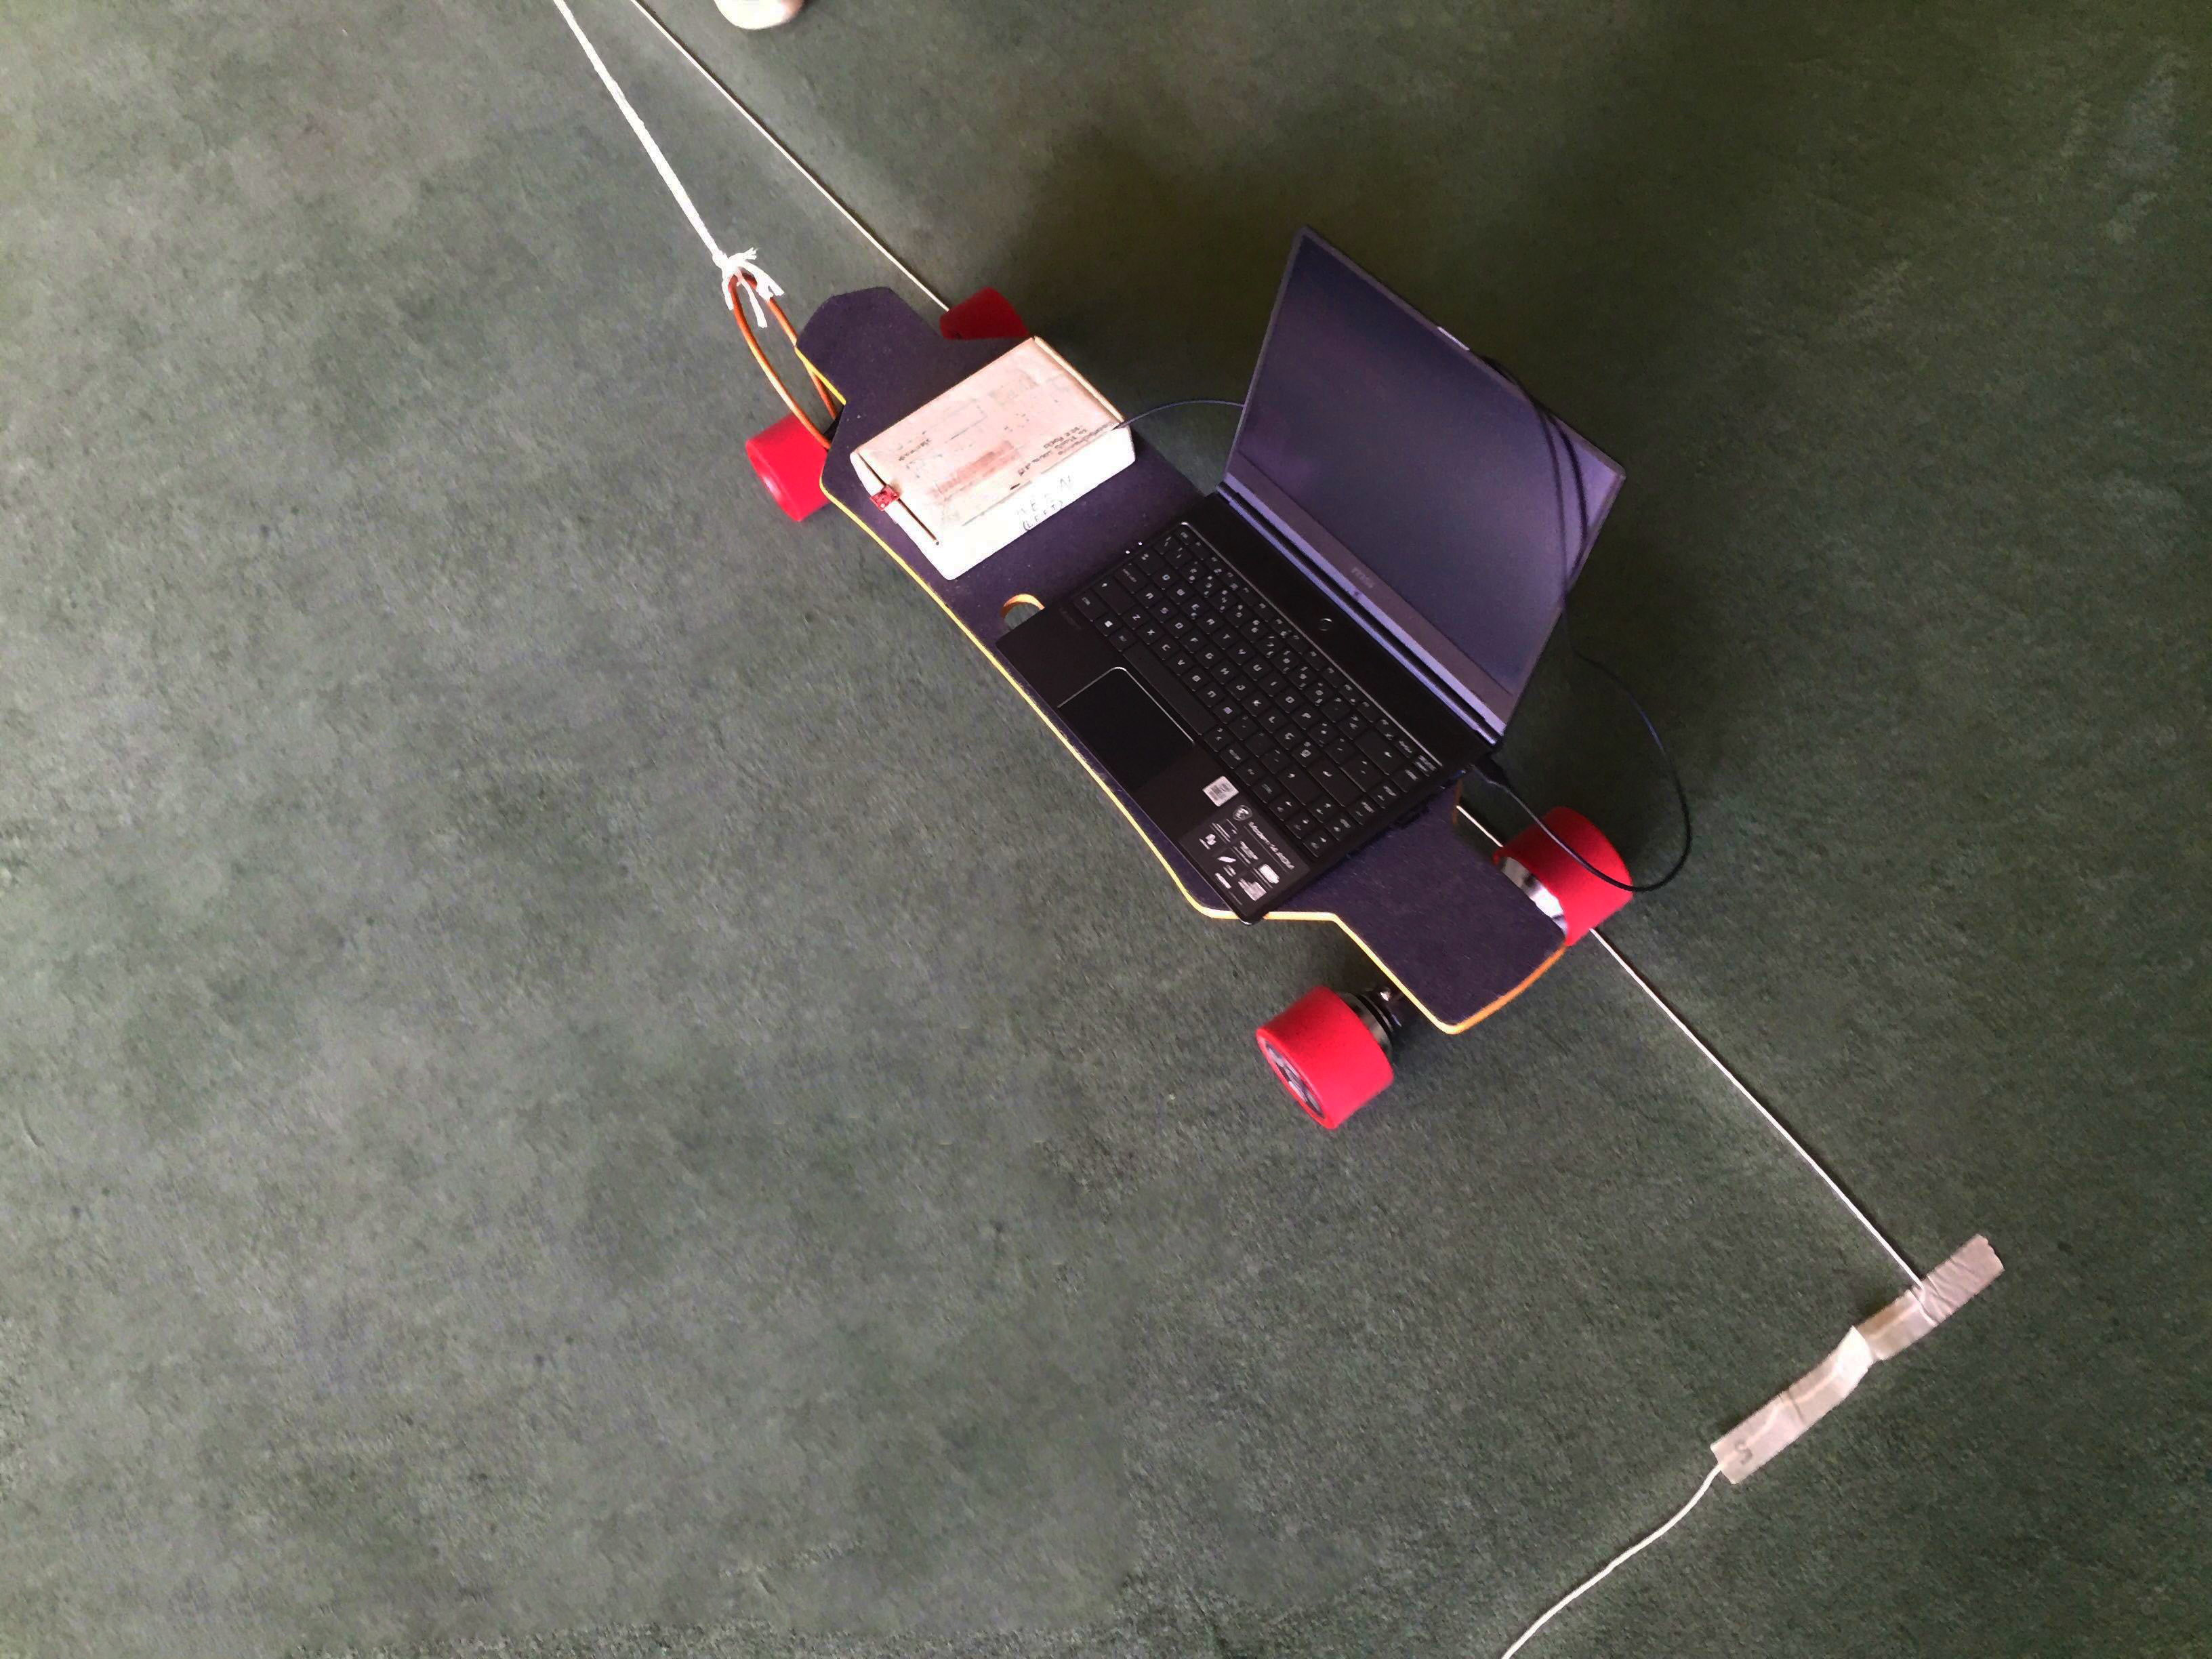
\includegraphics[width=0.9\textwidth]{figures/indoor_2.jpg}
    \caption{ Experiment made with skateboard to assess localization accuracy. }
    \label{fig:indoor_2}
\end{figure}

\subsection{Outdoor Experiments}
\begin{figure}[!h]
    \centering
    \includegraphics[width=0.9\textwidth]{figures/outdoor.jpg}
    \caption{ 5 meter side ground square used for baseline of accuracy of inertial system. }
    \label{fig:outdoor}
\end{figure}

\begin{figure}[!h]
    \centering
    \includegraphics[width=0.9\textwidth]{figures/outdoor_1.jpg}
    \caption{ Manually pulling the skateboard on each side of the ground square. }
    \label{fig:outdoor_1}
\end{figure}

\begin{figure}[!h]
    \centering
    \begin{subfigure}{0.49\textwidth}
        \centering
        \includegraphics[width=1\textwidth]{figures/outdoor_2.jpg}
        \caption{5 meter side ground square used for baseline of accuracy of inertial system.}
        \label{fig:outdoor_2}
    \end{subfigure}
    \begin{subfigure}{0.49\textwidth}
        \centering
        \includegraphics[width=1\textwidth]{figures/outdoor_3.jpg}
        \caption{ Manually pulling the skateboard on each side of the ground square. }
        \label{fig:outdoor_3}
    \end{subfigure}
    \caption{Pin connection between the microcontroller (left) and the IMU (right). Modules are linked through SCL, CLK, VDD and GND pins.}
    \label{fig:hardware}
\end{figure}